\documentclass{beamer}
\usepackage{graphicx}
\usepackage{listings} % Syntax highlighing
\usepackage{fancyvrb} % Inline verbatim
\usepackage{hyperref} % Hyperlinks
\hypersetup{pdfpagemode=FullScreen}
\usepackage{tikz}
\def\checkmark{\tikz\fill[scale=0.4](0,.35) -- (.25,0) -- (1,.7) -- (.25,.15) -- cycle;}

\usetheme{Boadilla}
\title{More Malware Models}
\author{UMBC Malware Data Science}
\date{Week 5: 25 February 2020}

\begin{document}

\begin{frame}{Recap}
    Last week, we discussed machine learning in general, and made Logistic Regression and Decision Tree models based on a few static features.
\end{frame}

\begin{frame}{Scientific Method}
    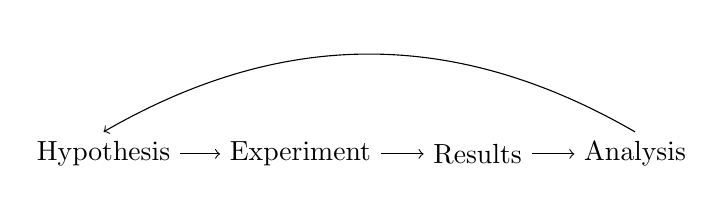
\begin{tikzpicture}
    % nodes
    \node (A) at (0, 0) {Hypothesis};
    \node (B) at (2.5, 0) {Experiment};
    \node (C) at (4.75, 0) {Results};
    \node (D) at (6.75, 0) {Analysis};
    
    % arrows
    \draw [->] (A) -- (B);
    \draw [->] (B) -- (C);
    \draw [->] (C) -- (D);
    \draw [->] (D.north) to [out=150,in=30] (A.north);
    \end{tikzpicture}
    \\ ~~ \\
    Our work with malware is the same:
    \begin{itemize}
        \item Results should be understandable by others.
        \item Results should be repeatable.
        \item Endgame's EMBER dataset \& the academic paper \textit{Variant: A Malware Similarity Testing Framework} offer common data for researchers to use to compare model accuracy.
        \item Here, we'll talk about algorithms and how to measure results to have a common language to discuss model performance.
        \begin{itemize}
            \item Otherwise: 
\includegraphics[scale=0.03]{Images/apple.jpg} $>$ 
\includegraphics[scale=0.04]{Images/orange.png}
        \end{itemize}
    \end{itemize}
\end{frame}

\begin{frame}{ML Algorithms}
    There's more to machine learning that just neural networks, and often the simpler model is more useful.
    \begin{itemize}
        \item Linear \& Logistic Regression: Fit a line between groups of data, recall $y=mx + b$ from elementary school, but with a lot more variables.
        \item Decision Trees: Branches of decision-making, if this then that... until we can learn class A vs. B.
        \item Support Vector Machines (SVM): Similar to above, attempts to draw a line (hyperplane) between the classes.
        \item Artificial Neural Networks: Mimicking the connections of neurons in the brain to develop ratios which model the data
        \begin{itemize}
            \item Deep Neural Networks (``Deep Learning''): Networks on top of networks, this is where a lot of image recognition, language modeling, and many other domains build their advanced models.
        \end{itemize}
        \item And there's others...
    \end{itemize}
    \small
    Remember: ``\textit{All models are wrong, but some are useful}'' -- George E. Box
\end{frame}

\begin{frame}{Decision Tree}
    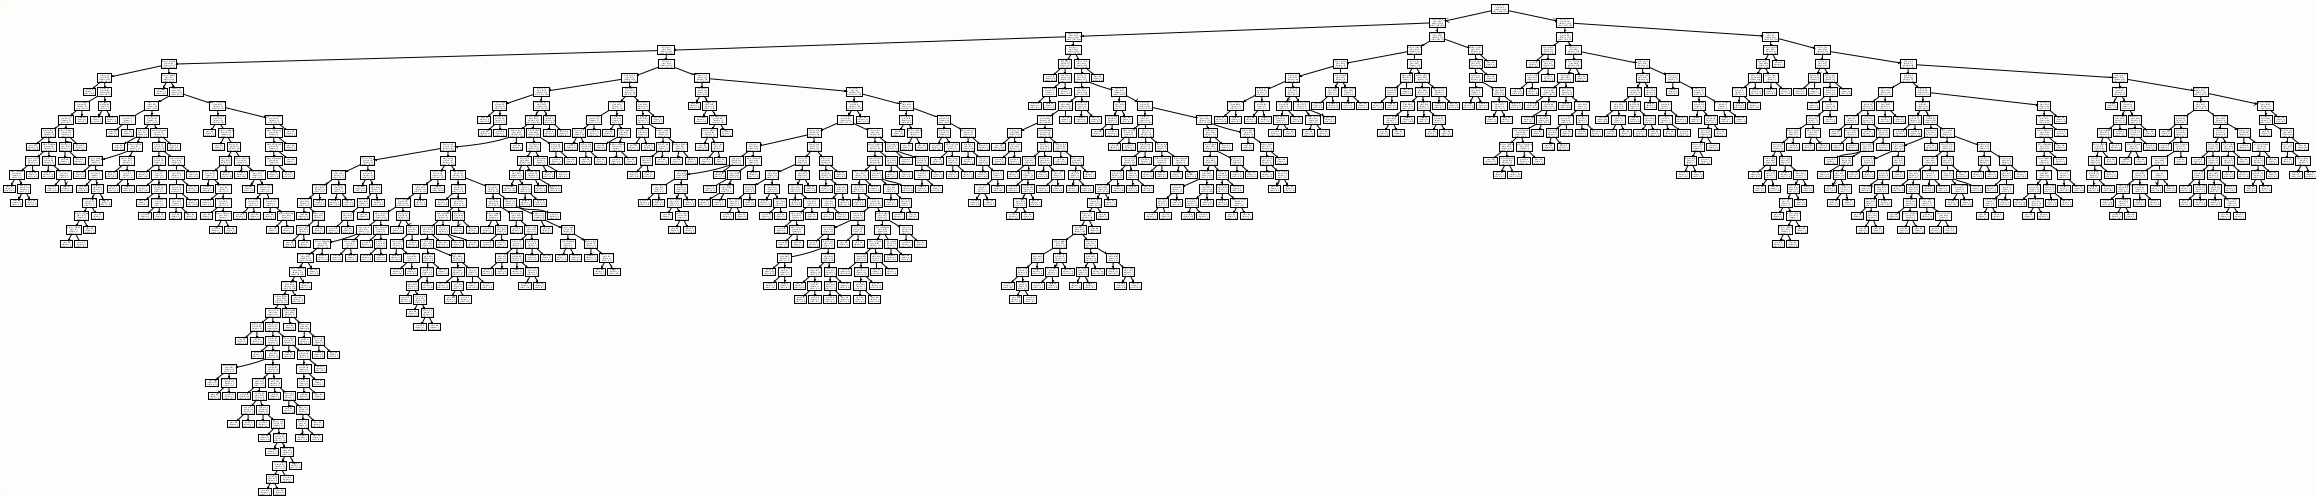
\includegraphics[scale=0.3]{Images/malware_decision_tree.png}
\end{frame}

\begin{frame}{Neural Network}
    \begin{columns}
        \column{0.55\textwidth} {
            \begin{itemize}
                \item Inputs are the features, outputs are malware or goodware in our case.
                \item The hidden nodes have initial random weights, which are multiplied by the input data, and the learning rate.
                \item During training, error information comes from the output to the hidden nodes to adjust it's internal weight value. This continues until the output is satisfactory.
                \item Due to randomness, the model will perform differently each time it's trained.
            \end{itemize}
        }
        \column{0.45\textwidth}{
            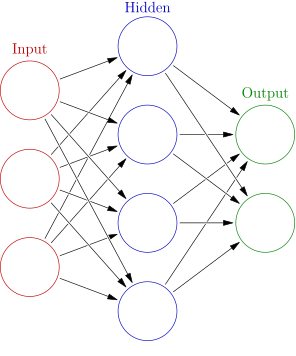
\includegraphics[scale=0.5]{Images/nn.png}
        }
   \end{columns}
\end{frame}

\begin{frame}
    \centering
    
\includegraphics[scale=0.52]{Images/deep_learning_meme.jpg}
\end{frame}

\begin{frame}{Measuring Results}
    \only<1>{
    When looking at the output of the model, there's more to consider than just accuracy.
    \begin{itemize}
        \item False Positives: Malware marked as benign
        \item False Negatives: Benign software marked malicious
        \item Recall $\frac{TP}{TP+FN}$: How much malware did we prevent from slipping by?
        \item Precision $\frac{TP}{TP+FP}$: How many of our malware predictions were actually malicious?
        \item F1 Score $2\frac{Recall * Precision}{Recall + Precision}$: Weighted average of above.
        \item ROC Curve (Receiver Operating Characteristics): Graph showing true positive rate vs. false positive rate.
        \item AUC (Area Under the [ROC] Curve): A class proportion-invariant way of measuring the effectiveness of a model.
        \item Fortunately all of this already exists in \texttt{sklearn}!
    \end{itemize}
    }
    \only<2>{
        When might some result measurements be preferred over others?
        \begin{itemize}
            \item A company making an anti-virus product probably wants a higher Precision score, since a lot of false positives will likely result in a busier support office \& fewer customers.
            \item A network defender, such as someone on the Blue Team, might be more interested in Recall, as that person wouldn't be upset by a higher degree of false positives, since they don't want any malware to get by.
        \end{itemize}
    }
\end{frame}

\begin{frame}{Example Results}
    98\% $\neq$ 98\%: Which would you pick? \\
     ~~ \\
    \begin{tabular}{ c c c c c }
     Actual\textbackslash Observed & Malware & Goodware & Accuracy:	& 98\% \\
     Malware & 1000 & 40 &  FP Rate: & 0 \\
     Goodware & 0   & 960 & FN Rate: & 0.04 \\
	           &     &    & Recall: & 0.96 \\
               &     & & Precision: & 1 \\ \hline
     Actual\textbackslash Observed & Malware & Goodware	& Accuracy:	& 98\% \\
     Malware & 980 & 20 &  FP Rate: & 0.02 \\
     Goodware & 20  & 980 & FN Rate:	& 0.02 \\
	          &      &     & Recall: & 0.98 \\
     Total Malware: & 1000 & & Precision: & 0.98 \\
     Total Goodware: & 1000	\\
    \end{tabular}
\end{frame}

\begin{frame}{ROC \& AUC}
    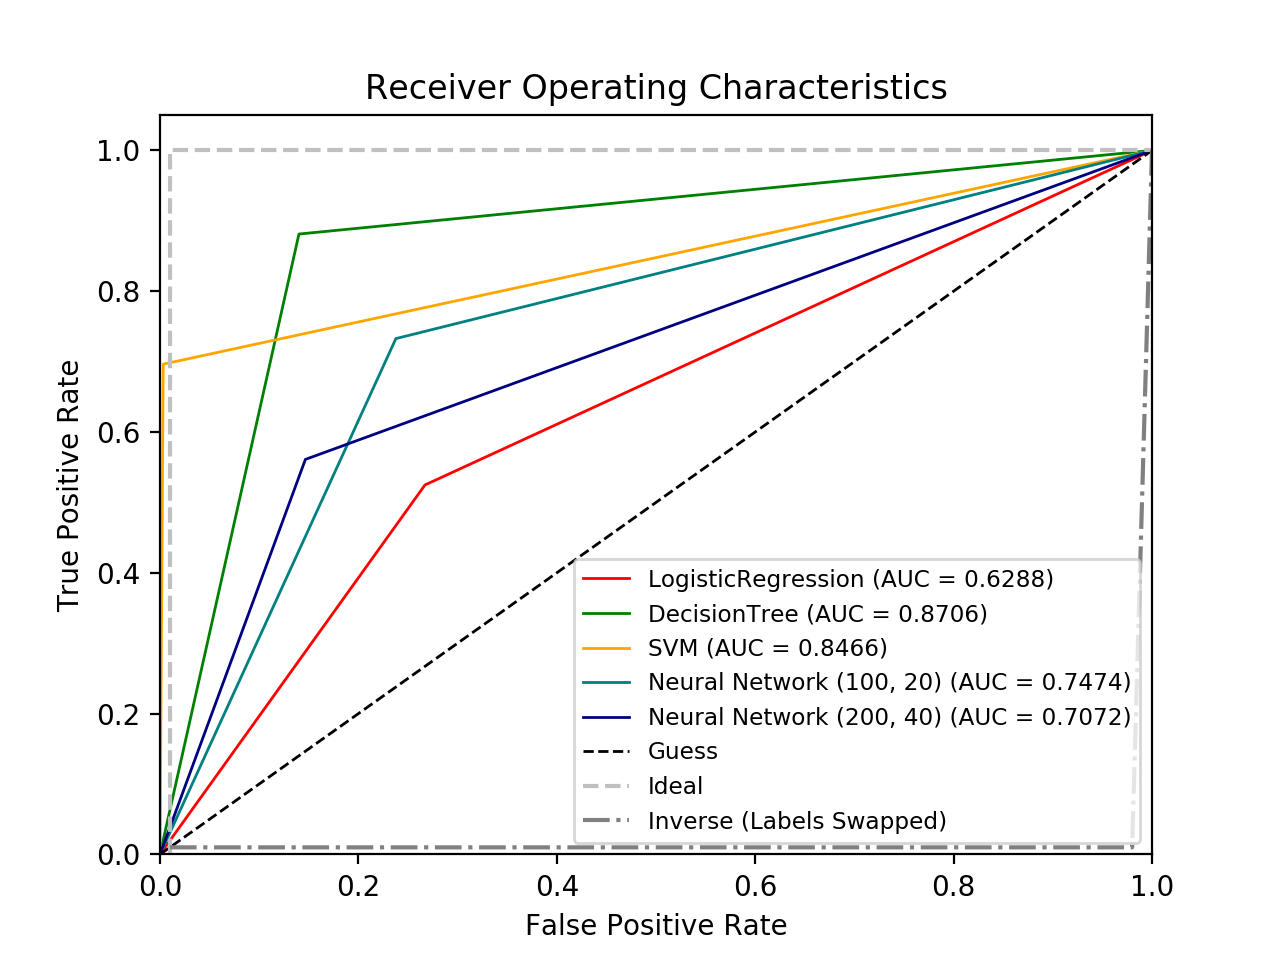
\includegraphics[scale=0.7]{Images/model_roc.png}
\end{frame}


\begin{frame}{Cross Validation}
    Another way to measure model performance is with $n$-fold cross validation. Instead of dividing the dataset into training and testing, the dataset is divided into several parts, with $n-1$ parts as training data, and one part as testing data. \\
    ~~ \\
    Train and test through the various combinations of the data, and save the model with the best performance, where the score type can be accuracy, AUC, F1, etc.
\end{frame}

\begin{frame}{Lab 5}
    For this Lab, we'll be using Endgame's EMBER dataset features with cross validation as implemented by sklearn to get the best model.
\end{frame}

\end{document}